\section{$\Delta$QSD concepts}

    We provide in this section the concepts needed to understand what is displayed on the oscilloscope.

\subsection{Representation of a $\Delta$Q}
    We provide a class to calculate the $\Delta$Q of a probe between a lower time bound $t_l$ and an upper time bound $t_u$. It can be calculated in two ways: 
    
    \paragraph{Observed $\Delta$Q}
    
    The first way is by having $n$ collected outcome instances between $t_l$ and $t_u$, calculating its \textit{probability density function} (PDF) and then calculating the \textit{empirical cumulative distribution function} (ECDF) based on its PDF. This is called the \textbf{Observed $\Delta$Q}.
    
    \paragraph{Calculated $\Delta$Q}
    
    A $\Delta$Q can also be calculated by performing operations on two or more observed $\Delta$Qs (convolution, operators operations), the notion of outcome instances is then lost between calculations, as the interest shifts towards calculating the resulting PDFs and ECDFs. This is called the \textbf{Calculated $\Delta$Q}. A simple outcome can \textbf{not} have a "calculated $\Delta$Q", we can only observe the delay from its observables.

    If you recall \cref{fig:probes_o}, the probes $p_2$ and $p_3$ observe simple outcomes, they can only display the observed $\Delta$Qs of $o_2, o_3$. The probe $p_1$ instead observes the sequential composition of said outcomes. We can display its "observed $\Delta$Q" from the execution from $start$ to $end$ and the "calculated $\Delta$Q" as the convolution of the observed $\Delta$Qs of $o_1, o_2$
        
    \begin{figure}[H]
            \begin{center}
                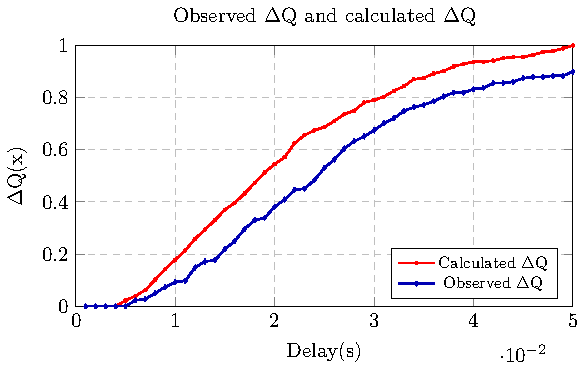
\includegraphics[scale=1]{tikz/obs_calc.pdf} 
            \end{center}
            \caption{(Red, circle, above): Calculated $\Delta$Q. (Blue, diamond, below): Observed $\Delta$Q}
        \end{figure}

    \subsection{dMax = $\Delta$t $\cdot$ N}
        The key concept of $\Delta$QSD is having a maximum delay after which we consider that the execution is timed out. This is represented in the oscilloscope as $dMax$. Understanding this equation is key to correctly using the oscilloscope and exploring tradeoffs

Setting a maximum delay for a probe is not a job that can be done one-off and blindly, it is something that is done with an underlying knowledge of the system inner-workings and must be thoroughly fine-tuned during the execution of the system by observing the resulting distributions of the obtained $\Delta$Qs. 

Let us explain the following equation:
\begin{equation}
    dMax = \Delta t \cdot N  
    \label{eq:dMaxU}
\end{equation}

    \begin{itemize}
        \item $dMax$: The maximum delay, it represents the maximum delay that an outcome instance of a probe can have. The execution is considered "timed out" (failure) after $dMax$.
        \item $\Delta t$: The resolution of a $\Delta$Q. It is the bin width of a bin in a probe's $\Delta$Q.
        \item $N$: The precision of a $\Delta$Q. It is the number of bins in a probe's $\Delta$Q.
    \end{itemize}
    
    It can be informally described as a "two out of three" equation. If the user wants higher precision but the same $dMax$, the resolution must change, and so on for every parameter.
        \begin{figure}[H]
            \centering
            \begin{subfigure}{.5\textwidth}
                \centering
                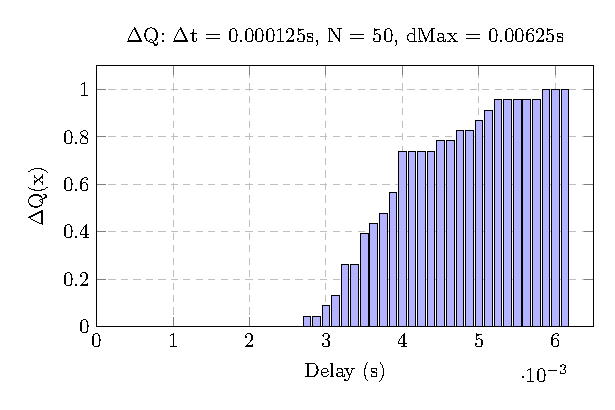
\includegraphics[width =0.98\textwidth]{tikz/hist_50.pdf}
                \label{fig:hist_50}
            \end{subfigure}%
            \begin{subfigure}{.5\textwidth}%
                \centering%
                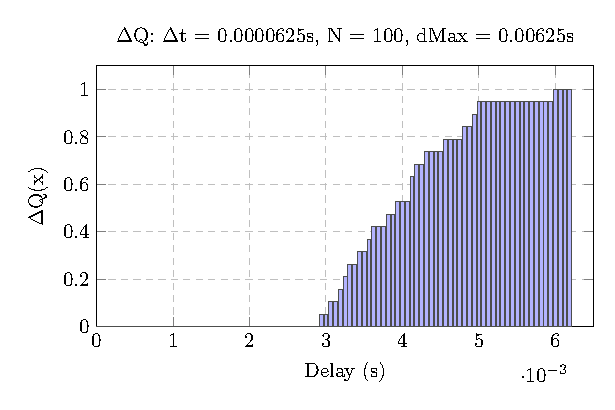
\includegraphics[width =0.98\textwidth]{tikz/hist_100.pdf}%
                \label{fig:hist_100}%
            \end{subfigure}%
            \label{fig:hist_dmax}%
            \caption{Left: Sample $\Delta$Q representation as a histogram with higher resolution but lower precision. \\
            Right: Sample $\Delta$Q representation as a histogram with lower resolution but higher precision. \\
            Both $\Delta$Qs have the same $dMax$, but the amount of precise information they provide is far different.}
        \end{figure}%

Some tradeoffs must though be acknowledged when setting these parameters, a higher number of bins corresponds to a higher number of calculations and space complexity, a lower $dMax$ may correspond to more failures. The user must set these parameters carefully during execution y observing the shown plots.

    \begin{figure}[H]
        \begin{center}
            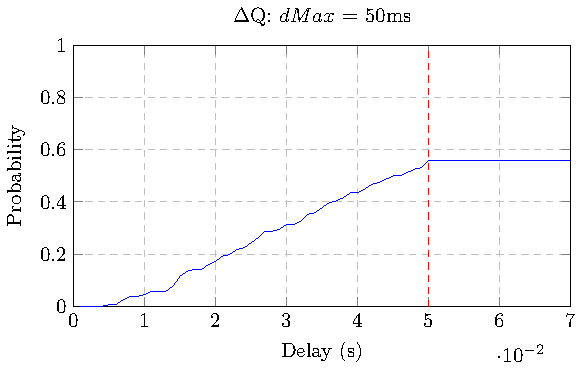
\includegraphics[scale = 1]{tikz/cdf_dmax.pdf}
        \end{center}
        \caption{$\Delta$Q: $dMax$ = 50ms, the $\Delta$Q will stay constant when delay $> dMax$.}
    \end{figure}

    \subsubsection{dMax limitation}
        $dMax$ can \textbf{not} be lower than 1 millisecond and will be rounded to the \textbf{nearest} integer in the adapter, this is a limitation of Erlang \texttt{send\_after} function which only accepts integers and milliseconds values. For example, if on the oscilloscope the $dMax$ is equal to $1.56 ms$, the adpater will fail spans after 2 ms.

    \subsection{QTA}
        A simplified QTA is defined for probes. We define 4 points for the step function at 25, 50, 75 percentiles and the maximum amount of failures accepted for an observable. An observed $\Delta$Q will calculate that based on the samples collected. 

\subsection{Confidence bounds}
    To observe the stationarity of a probe we must observe its $\Delta$Qs over a polling window and calculate confidence bounds over said $\Delta$Qs. A single $\Delta$Q may fluctuate, moreover, as it is an ECDF, it is not as precise as a CDF and, based on the number of bins, may not be precise. This is why we include the mean and confidence bounds of $\Delta$Qs in the plot.

    We first calculate a mean of the $\Delta$Qs in the polling window, this gives an idea of how the probe has been behaving during the polling window. \\
    Given this mean, we can calculate its confidence bounds, which give a probability range over which the true CDF of the $\Delta$Q should fall. \cite{conf-b}

    The bounds are updated dynamically by inserting or removing a $\Delta$Q. Every time a new $\Delta$Q is calculated, the oldest $\Delta$Q in a window is removed if \#$\Delta$Qs(polling window) $>$ limit. The new $\Delta$Q is added to the calculation of the mean and confidence bounds as it is calculated. \\
    This allows us to consider a small window of execution rather than observing the execution since the start for the bounds, this can help in observing stationarity of the system, where less sampled $\Delta$Qs can help observe short term behaviour. \\
    With a big window of $\Delta$Qs, temporary overload may not greatly affect the mean and bounds, while, if we consider the current size of the polling window (30 $\Delta$Qs), a few $\Delta$Qs which deviate from stationary behaviour have a greater impact on the bounds and mean.
        \begin{figure}[H]
            \begin{center}
                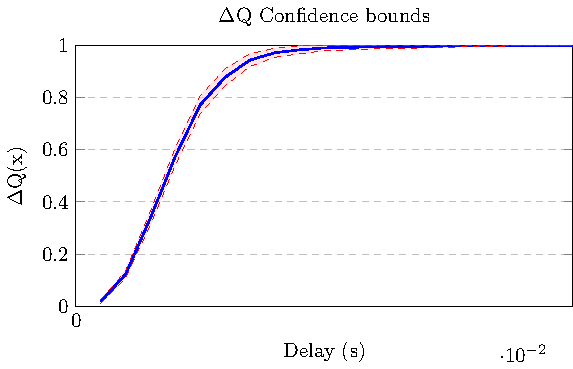
\includegraphics[scale=1]{tikz/ci.pdf} 
            \end{center}
            \caption{Upper and lower bounds (dashed, red) of the mean (blue) of multiple $\Delta$Qs. In a system that behaves linearly, the bounds will be close to the mean, once the overload is approaching, or a system is showing behaviour that diverges from a linear one, the bounds will appear larger.}
        \end{figure}

  
